\chapter{Especificación de Requisitos}
\title{Especificación de Requisitos}

\paragraph{
Para lograr que el desarrollo de un sistema hardware o software sea un éxito, es necesario que los desarrolladores comprendan totalmente las especificaciones que requiere el proyecto. En esta sección se va a proceder a enumerar los requisitos del sistema en el que se está trabajando.
}

\title{Modelado del sistema}
\section{
Modelado del sistema
}

\paragraph{
El dispositivo que se desea desarrollar tiene que hacer la función básica del director de la banda de música durante una actuación, es decir, marcar el mismo pulso a los músicos.
}

\paragraph{
Cuando la agrupación se encuentra realizando un concierto, el
esquema de comunicación que se sigue es el mostrado en la figura \ref{fig:modeladoconceptual}
(donde el nodo rojo es el director y lo morados los músicos). El único flujo de información
que hay es que que marcan las flechas (el pulso, que sigue un tempo constante). Hay que
aclarar que en este caso, para simplificar, sólo se han dibujado 5 músicos,
sin embargo, como se vio en la introducción, las bandas suelen contar entre sus filas con
varias decenas de integrantes.
}

\begin{figure}[htb]
\centering
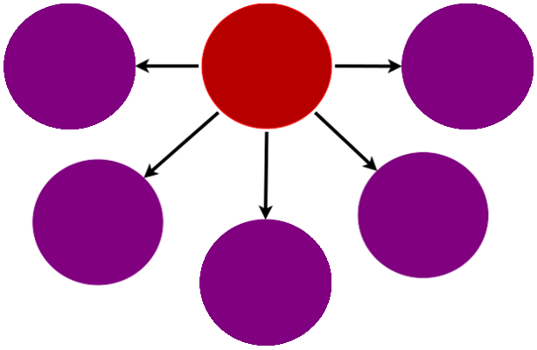
\includegraphics[width=0.6\textwidth]{./imagenes/modeladoconceptual}
\caption{Modelado del sistema} \label{fig:modeladoconceptual}
\end{figure}

\paragraph{
La información que se envía es la siguiente:
}
  \begin{figure}[htb]
  \centering
  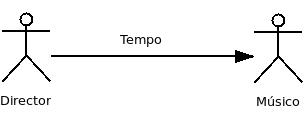
\includegraphics[width=0.6\textwidth]{./imagenes/mensajesconceptual}
  \caption{Traspaso de información} \label{fig:mensajesconceptual}
  \end{figure}


\paragraph{
Como se puede apreciar, no es necesario guardar ningún tipo de información sobre los músicos o el director. Tan solo
es necesario guardar el ``tempo'' (que será establecido por el director).
}

\title{Actores}
\section{Actores}

\paragraph{
Del esquema de la figura \ref{fig:mensajesconceptual} podemos sacar una conclusión clara:
será necesaria la distinción entre dos usuarios en nuestro sistema,
}
  \begin{itemize}
    \item Director: es el que envía el pulso al resto de actores. Solo uno por sistema
    \item Músico: recibe el pulso del director. Habrá multiples
  \end{itemize}


\title{Requisitos funcionales}
\section{Requisitos funcionales}

\paragraph{
En este apartado se van a describir los requisitos funcionales del sistema.
Estos requisitos son aquellas funciones o capacidades que el sitema debe
tener para satisfacer las necesidades de los usuarios.
}

\begin{itemize}
    \item[\textbf{RF.1}] El sistema permitirá al director insertar un tempo
    \item[\textbf{RF.2}] Se capacitará al director para hacer llegar el pulso adecuado a los intérpretes
    \item[\textbf{RF.3}] El pulso se comunicará a los músicos a través de algún actuador (una señal visual, por ejemplo)
\end{itemize}


\title{Requisitos no funcionales}
\section{Requisitos no funcionales}

\paragraph{
En estea sección se van a describir los distintos requisitos no funcionaels del sistema.
Los requisitos no funcionales son aquellos que nos informan de restricciones que debe cumplir
nuestro sistema.
}

\begin{itemize}
    \item[\textbf{RNF.1}] El sistema debe ser wireless
    \item[\textbf{RNF.2}] Debe de ser barato
    \item[\textbf{RNF.3}] La escalabilidad no debe ser un problema
    \item[\textbf{RNF.4}] Debe permitir que se puedan añadir funciones
    \item[\textbf{RNF.5}] El dispositivo que se desarrolle tiene que ser discreto y cómodo
    \item[\textbf{RNF.6}] Bajo consumo energético
\end{itemize}
